% \section{Methodology}

% \subsection{Dataset and Preprocessing}

% We use a subset of the YouTube-8M dataset (May 14, 2018 version)~\cite{abu2016youtube}. Our working set consists of approximately 1,800 videos, categorized into 10 distinct classes, with each video averaging around 20 seconds in length. The dataset is split into training, validation, and test sets following an 8:1:1 ratio.

% Data preprocessing involved downloading video shards, sampling a subset of videos, and extracting a variety of features. For each video, we obtained both raw and embedded representations, including:

% \begin{itemize}
%     \item \textbf{Audio Features}: 1024-dimensional embeddings generated using the TwelveLabs embedding API~\cite{jung2024pegasus, lee2024twlv}.
%     \item \textbf{Video-Text Features}: 1024-dimensional embeddings also derived from the TwelveLabs embedding API~\cite{jung2024pegasus, lee2024twlv}.
%     \item \textbf{Metadata Embeddings}: 3072-dimensional embeddings produced by OpenAI’s \texttt{text-embedding-3-large} model, applied to textual metadata such as video tags.
% \end{itemize}

% All extracted features and embeddings were serialized into individual HDF5 files to support efficient data loading during training and evaluation. To verify the quality of the embeddings, we employed UMAP~\cite{mcinnes2018umap} for dimensionality reduction. The resulting visualizations demonstrate clear separability among the video classes, as illustrated in Figure~\ref{fig:umap}.

% \begin{figure}[h]
% \begin{center}
%    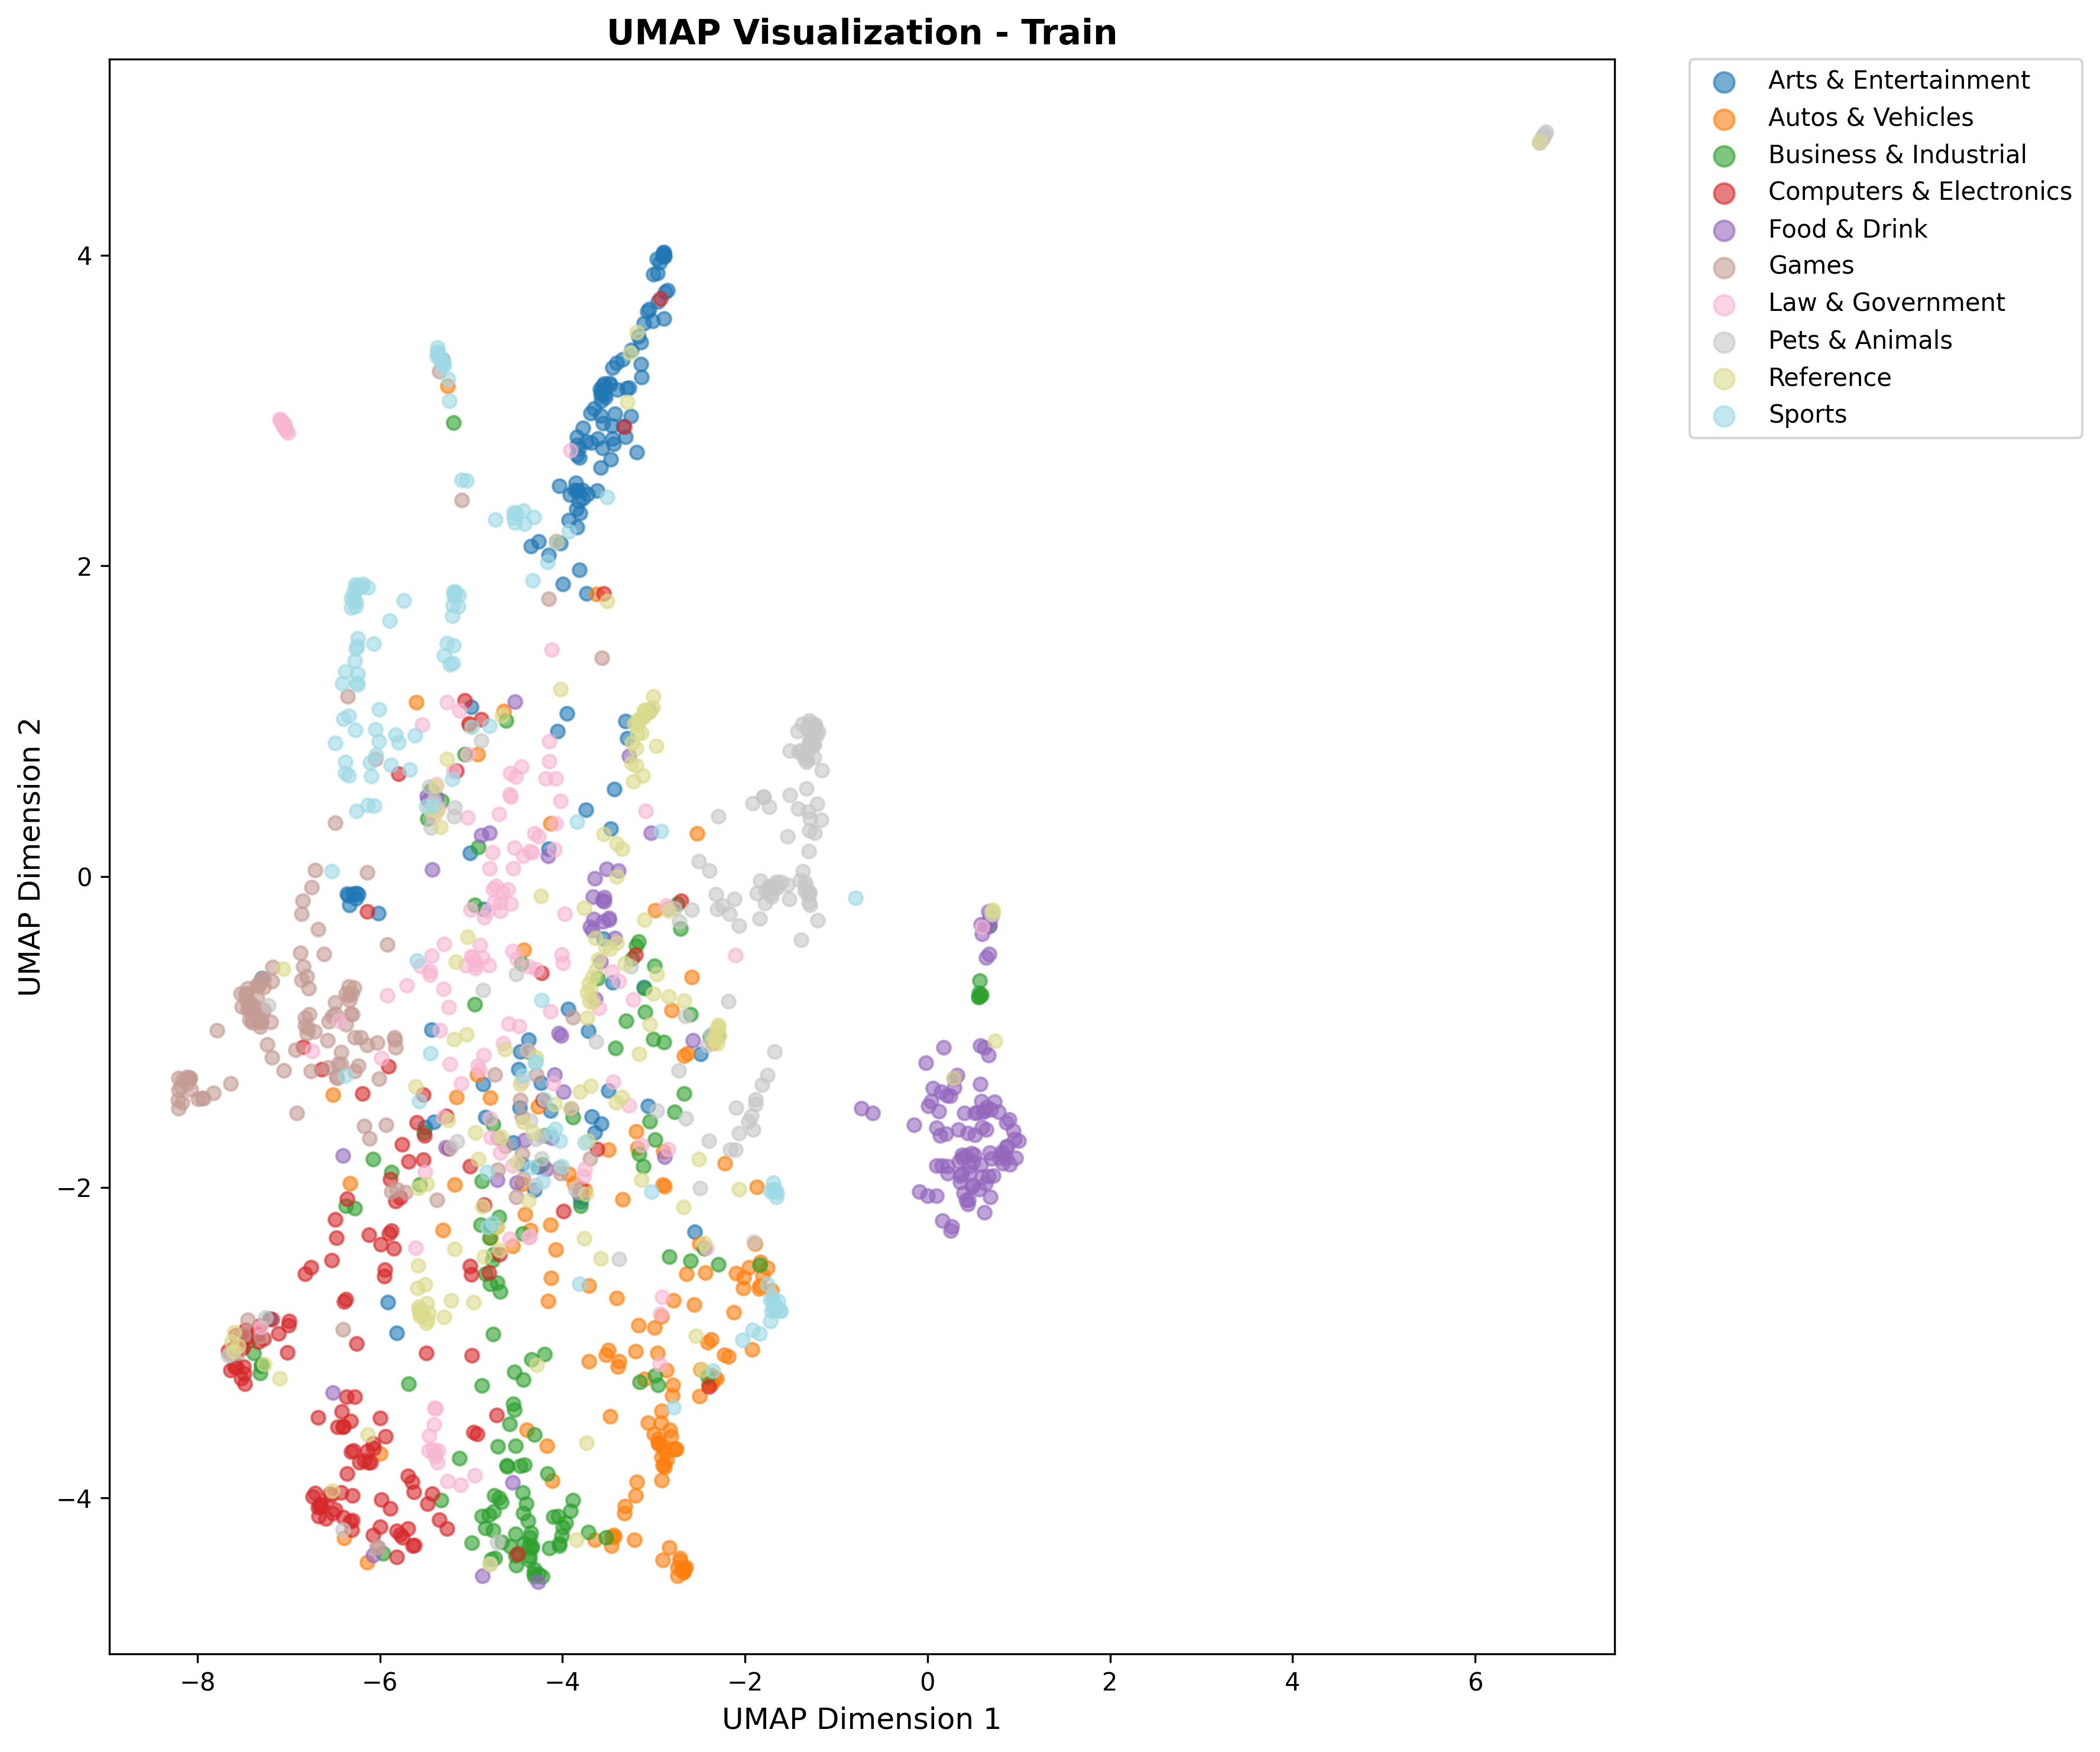
\includegraphics[width=0.8\linewidth]{asset/umap_train.png}
% \end{center}
%    \caption{UMAP visualization of video embeddings from the training set, showing distinct clustering by class.}
% \label{fig:umap}
% \end{figure}


% \subsection{Baseline Models}
% We established two baseline models for comparison:
% \begin{itemize}
%     \item \textbf{Zero-Shot Classification}: Using pre-trained embeddings without any fine-tuning on our dataset, this approach achieved an accuracy of 55.6%[cite: 10, 11].
%     \item \textbf{TimeSformer-Based Classification}: We fine-tuned a TimeSformer model (pre-trained on Kinetics-400\cite{kay2017kinetics}) on our dataset. This model achieved 64.0% accuracy after approximately 10 hours of training[cite: 13].
% \end{itemize}

% \subsection{Proposed Method}
% Our proposed method involves a neural network that takes concatenated multimodal embeddings as input. The architecture consists of a Multi-Layer Perceptron (MLP) followed by a classification layer. Key training parameters include 20 epochs, a batch size of 8, and a CosineAnnealingLR scheduler~\cite{loshchilov2016sgdr}, leading to a total training time of approximately 1 minute.

% \textbf{Data Augmentation}: We introduce a novel data augmentation technique applied directly to the embeddings. Noise is generated, normalized, scaled by an augmentation strength, added to the original embedding, and then the result is re-normalized. This helps to prevent overfitting and improve generalization, particularly in the cosine distance space where these embeddings often operate. 
% % Equation for augmentation could be added here if space allows:
% \[
% noise = strength * gaussian\_noise / ||gaussian\_noise||_2
% \]
% \[
% emb_{aug} = (emb + noise ) / ||emb + noise||_2 
% \]
% The augmentation process is illustrated in Figure~\ref{fig:augmentation}
% \begin{figure}[h]
% \begin{center}
%    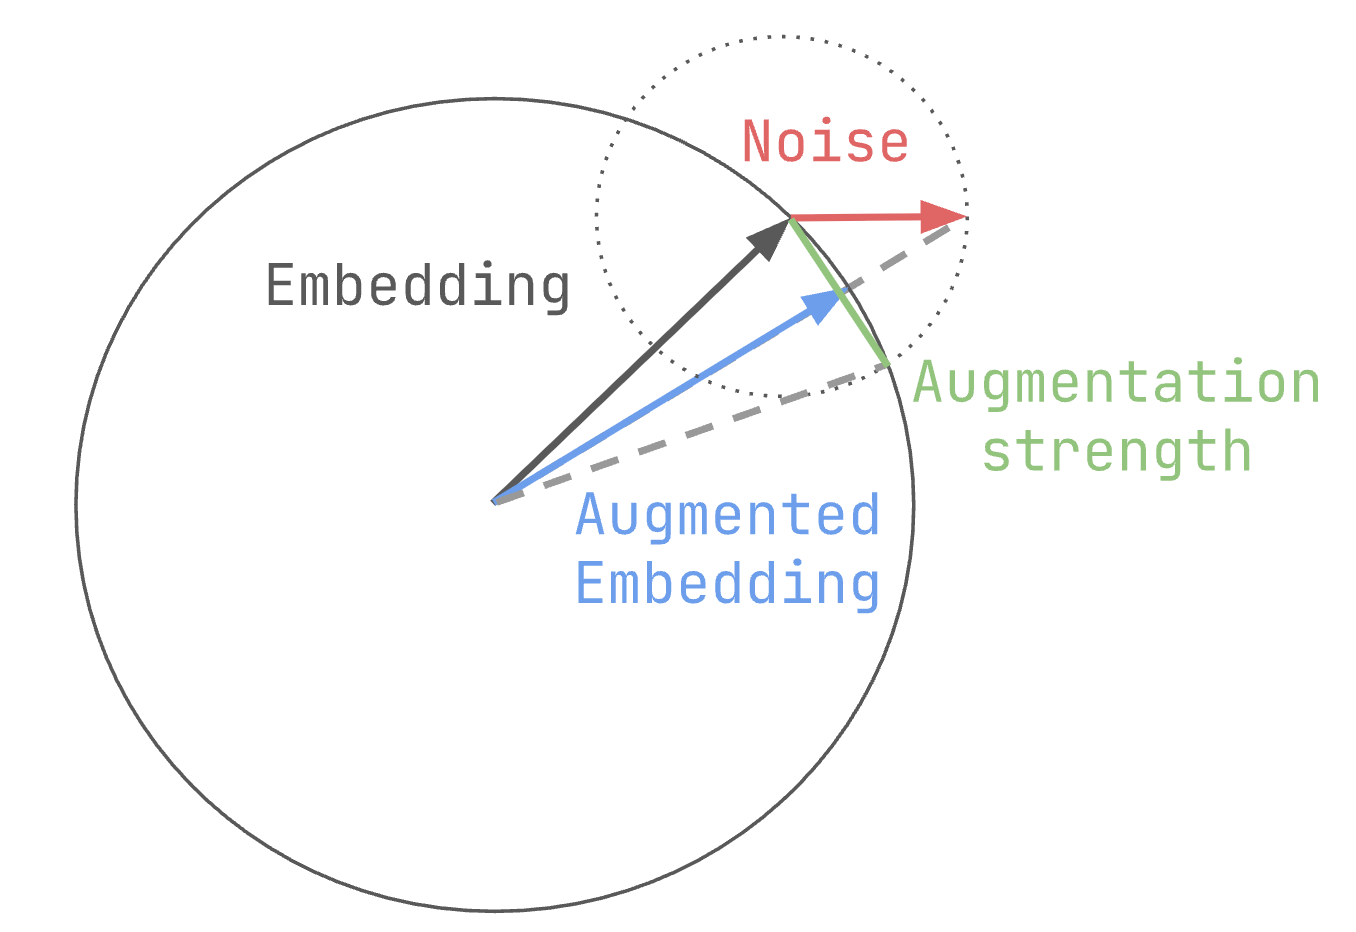
\includegraphics[width=0.8\linewidth]{asset/augmentation.png}
% \end{center}
%    \caption{Data augmentation process on cosine distance space.}
% \label{fig:augmentation}
% \end{figure}


% \section{Methodology}

% \subsection{Dataset and Preprocessing}

% We utilize a subset of the YouTube-8M dataset (May 14, 2018 version)~\cite{abu2016youtube}, comprising approximately 1,800 videos categorized into 10 distinct classes. Each video has an average duration of around 20 seconds. The dataset is divided into training, validation, and test splits using an 8:1:1 ratio.

% Preprocessing involved downloading video shards, sampling the working subset, and extracting various features. For each video, both raw and embedded representations were obtained, including:

% \begin{itemize}
%     \item \textbf{Audio Features}: 1024-dimensional embeddings generated using the TwelveLabs embedding API~\cite{jung2024pegasus, lee2024twlv}.
%     \item \textbf{Video-Text Features}: 1024-dimensional embeddings also produced via the TwelveLabs embedding API~\cite{jung2024pegasus, lee2024twlv}.
%     \item \textbf{Metadata Embeddings}: 3072-dimensional embeddings derived from OpenAI’s \texttt{text-embedding-3-large} model, applied to textual metadata such as video tags.
% \end{itemize}

% All features were serialized into individual HDF5 files to enable efficient loading during training and evaluation. To assess the quality of the embeddings, we employed UMAP~\cite{mcinnes2018umap} for dimensionality reduction. The resulting visualizations, shown in Figure~\ref{fig:umap}, reveal clear class-wise separability.

% \begin{figure}[h]
% \begin{center}
%    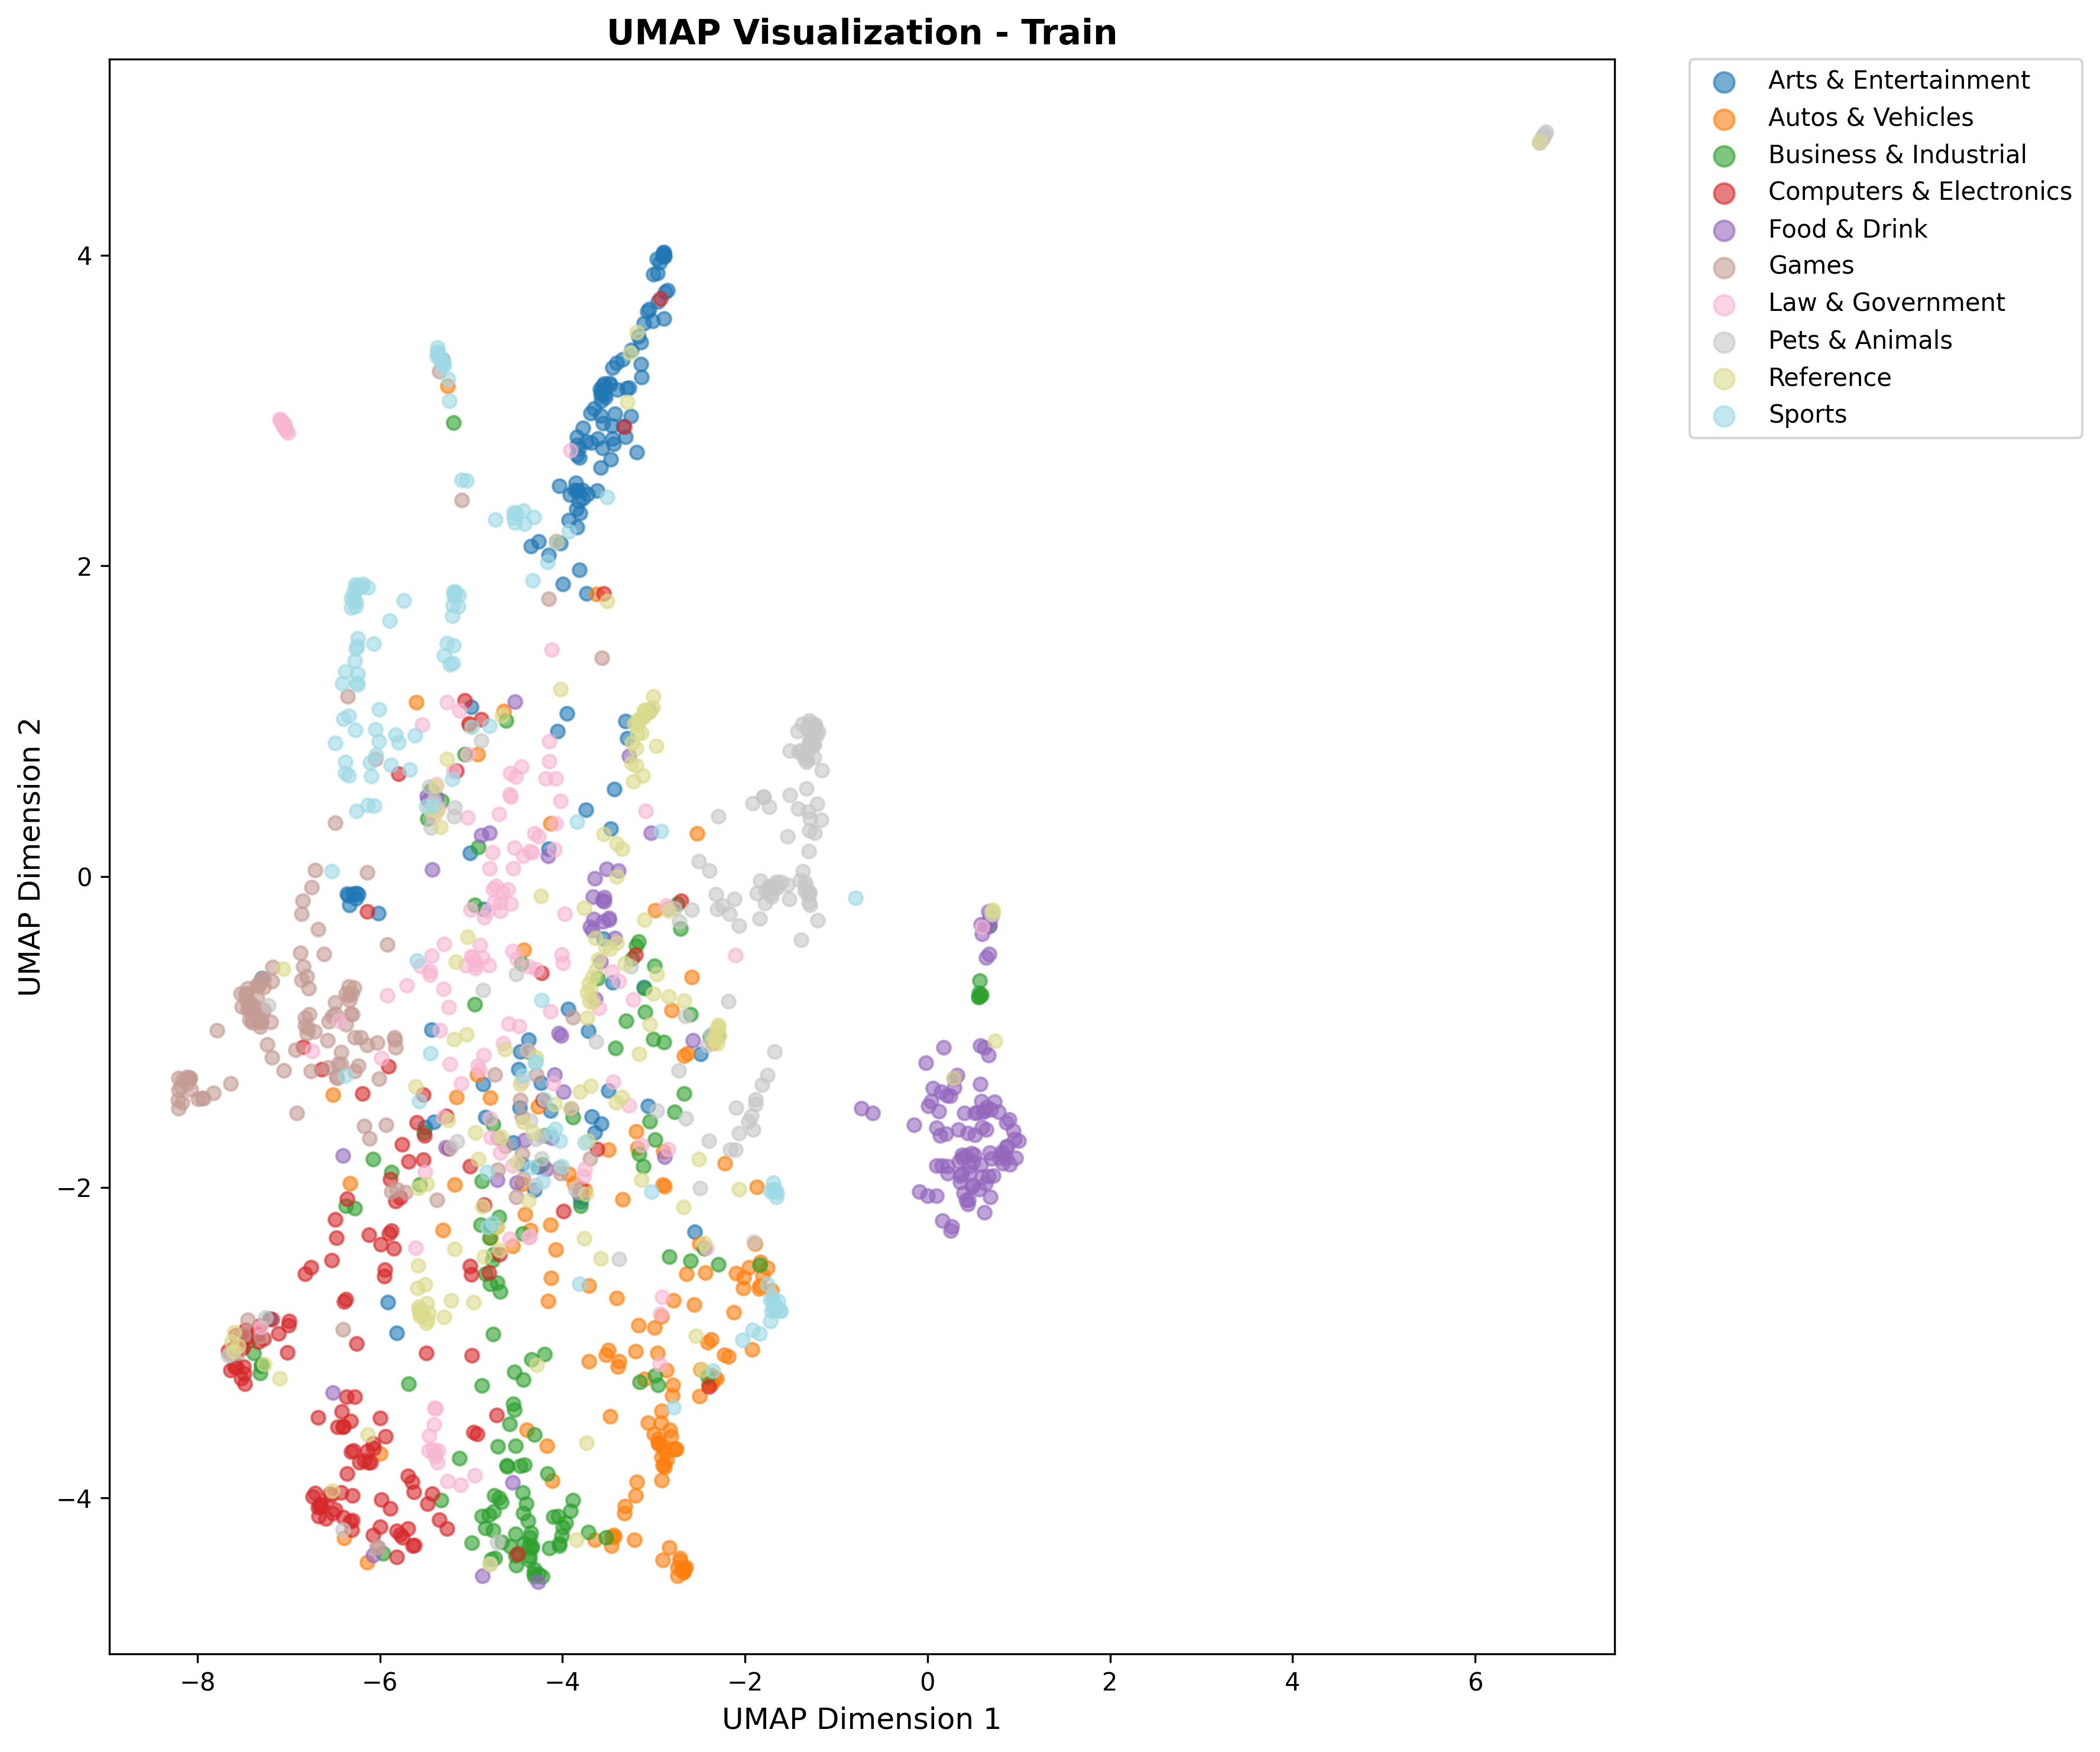
\includegraphics[width=0.8\linewidth]{asset/umap_train.png}
% \end{center}
%    \caption{UMAP visualization of training set video embeddings, illustrating distinct clusters corresponding to different classes.}
% \label{fig:umap}
% \end{figure}

% \subsection{Baseline Models}

% We implemented two baseline models for performance comparison:

% \begin{itemize}
%     \item \textbf{Zero-Shot Classification}: With TwelveLabs video embeddings and text embeddings without any training. It achieved an accuracy of 55.6\%.
    
%     \item \textbf{TimeSformer-Based Classification}: We fine-tuned a TimeSformer model pre-trained on the Kinetics-400 dataset~\cite{kay2017kinetics} using our dataset. This model attained 64.0\% accuracy after approximately 10 hours of training~.
% \end{itemize}

% \subsection{Proposed Method}

% Our proposed model utilizes a neural network that ingests concatenated multimodal embeddings as input. The architecture is composed of a Multi-Layer Perceptron (MLP) followed by a classification head. Key training parameters include 20 epochs, a batch size of 8, and a CosineAnnealingLR scheduler~\cite{loshchilov2016sgdr}, with a total training time of approximately one minute.

% \textbf{Data Augmentation}: To enhance generalization and mitigate overfitting, we introduce a novel augmentation method directly applied to the embeddings. The process involves generating Gaussian noise, normalizing it, scaling it by a configurable strength parameter, adding it to the original embedding, and then re-normalizing the result. This is particularly beneficial in the cosine distance space where these embeddings are typically used.

% The augmentation is defined as:
% \[
% \text{noise} = \text{strength} \times \frac{\text{gaussian\_noise}}{\|\text{gaussian\_noise}\|_2}
% \]
% \[
% \text{emb}_{\text{aug}} = \frac{\text{emb} + \text{noise}}{\|\text{emb} + \text{noise}\|_2}
% \]
% This augmentation process guarantee the augmented embeddings in cosine distance smaller than $1 -  \sqrt{1 - strength ^2}$ with original embedding.
% The augmentation process is illustrated in Figure~\ref{fig:augmentation}.

% \begin{figure}[h]
% \begin{center}
%    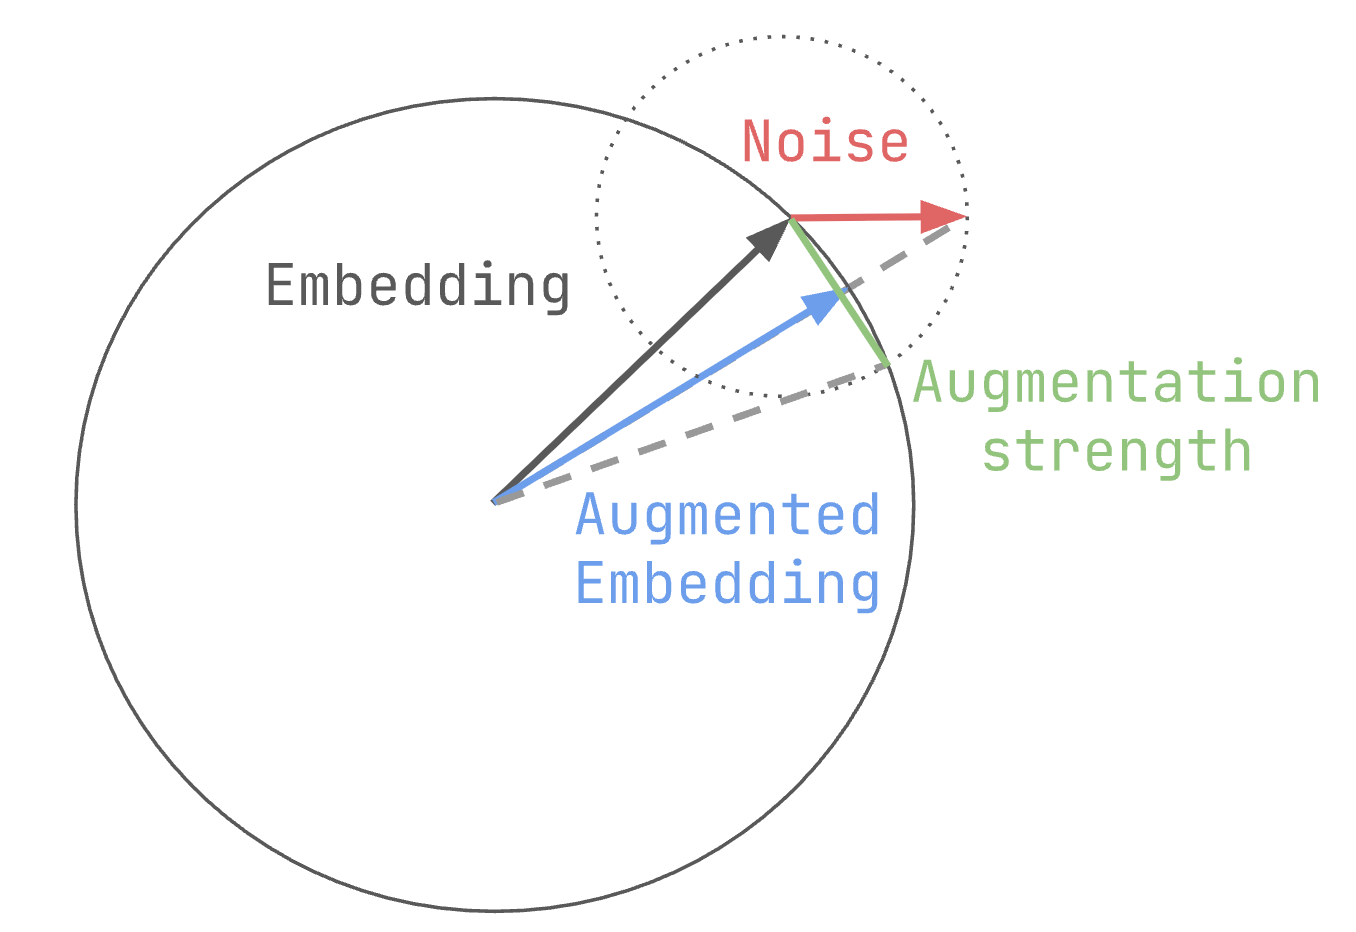
\includegraphics[width=0.8\linewidth]{asset/augmentation.png}
% \end{center}
%    \caption{Illustration of the data augmentation technique in cosine distance space.}
% \label{fig:augmentation}
% \end{figure}

\section{Methodology}

\subsection{Dataset and Preprocessing}

%We use a subset of the YouTube-8M dataset (May 14, 2018 version)~\cite{abu2016youtube}, consisting of approximately 1,800 videos spanning 10 classes. Each video is, on average, about 20 seconds long. We split the data into training, validation, and test sets in an 8:1:1 ratio.

%Preprocessing proceeds as follows:

The present study utilizes a subset of the YouTube-8M dataset (May 14\textsuperscript{th}, 2018 version)~\cite{abu2016youtube}, consisting of approximately 1,800 videos spanning 10 classes: \textit{Arts \& Entertainment}, \textit{Autos \& Vehicles}, \textit{Business \& Industrial}, \textit{Computers \& Electronics}, \textit{Food \& Drink}, \textit{Games}, \textit{Law \& Government}, \textit{Pets \& Animals}, \textit{Reference}, and \textit{Sports}.
The duration of each video is approximately 20 seconds on average.
The data was then divided into training, validation and test sets in an 8:1:1 ratio.

The preprocessing procedure is outlined as follows:

%\begin{enumerate}
    %\item Download the full YouTube-8M video shards.
    %\item Sample the working subset of 1,800 videos (balanced across the 10 classes).
    %\item For each video, extract and save:
    %\begin{itemize}
        %\item \textbf{Audio Embeddings}: 1,024-dimensional vectors via the TwelveLabs embedding API~\cite{jung2024pegasus, lee2024twlv}.
        %\item \textbf{Video–Text Embeddings}: 1,024-dimensional vectors via the TwelveLabs embedding API~\cite{jung2024pegasus, lee2024twlv}.
        %\item \textbf{Metadata Embeddings}: 3,072-dimensional vectors computed by applying %OpenAI’s \texttt{text-embedding-3-large} model~\cite{openai_text_embedding_3_large} to textual metadata (e.g., video tags).
    %\end{itemize}
    %\item Serialize all embeddings into individual HDF5 files for efficient loading during %training and evaluation.
%\end{enumerate}

\begin{enumerate}
    \item YouTube-8M dataset video shards are downloaded.
    \item The working subset of 1,800 videos, balanced across the 10 classes, is sampled.
    \item For each video, the following embeddings are extracted:
    \begin{itemize}
        \item \textbf{Video\-Text and Audio Embeddings}: The TwelveLabs embedding API~\cite{lee2024twlv, twelvelabs_embed_api_doc} facilitates the extraction of 1,024-dimensional vectors.
        \item \textbf{Metadata Embeddings}: A total of 3,072-dimensional vectors have been computed by applying OpenAI's \texttt{text-embedding-3-large} model~\cite{openai_text_embedding_3_large} to textual metadata, such as video tags.
    \end{itemize}
    \item All embeddings are serialized into individual HDF5 files, thus ensuring efficient loading during the training and evaluation phases.
\end{enumerate}

%To verify that the pretrained embeddings exhibit class-wise structure, we apply UMAP~\cite{mcinnes2018umap} to reduce the dimensionality of the video–text embeddings. As shown in Figure~\ref{fig:umap}, the resulting 2D projection reveals clear clusters corresponding to different classes.

Videos are additionally processed to meet the resolution and aspect ratio requirements defined by the TwelveLabs Embed API.
Specifically, a Python module leveraging the MoviePy library assesses each video's original resolution and aspect ratio, resizing and padding the videos to align with the nearest allowed dimensions (e.g., 1:1, 4:3, 16:9).
This ensures all videos consistently meet API specifications, streamlining the embedding extraction process.

To verify that the pretrained embeddings exhibit class-wise structure, the Unsupervised Manifold Alignment Projection (UMAP)~\cite{mcinnes2018umap} algorithm is applied to reduce the dimensionality of the video-text embeddings.
As demonstrated in Figure~\ref{fig:umap}, the resulting 2D projection reveals distinct clusters corresponding to different classes.

\begin{figure}[h]
\centering
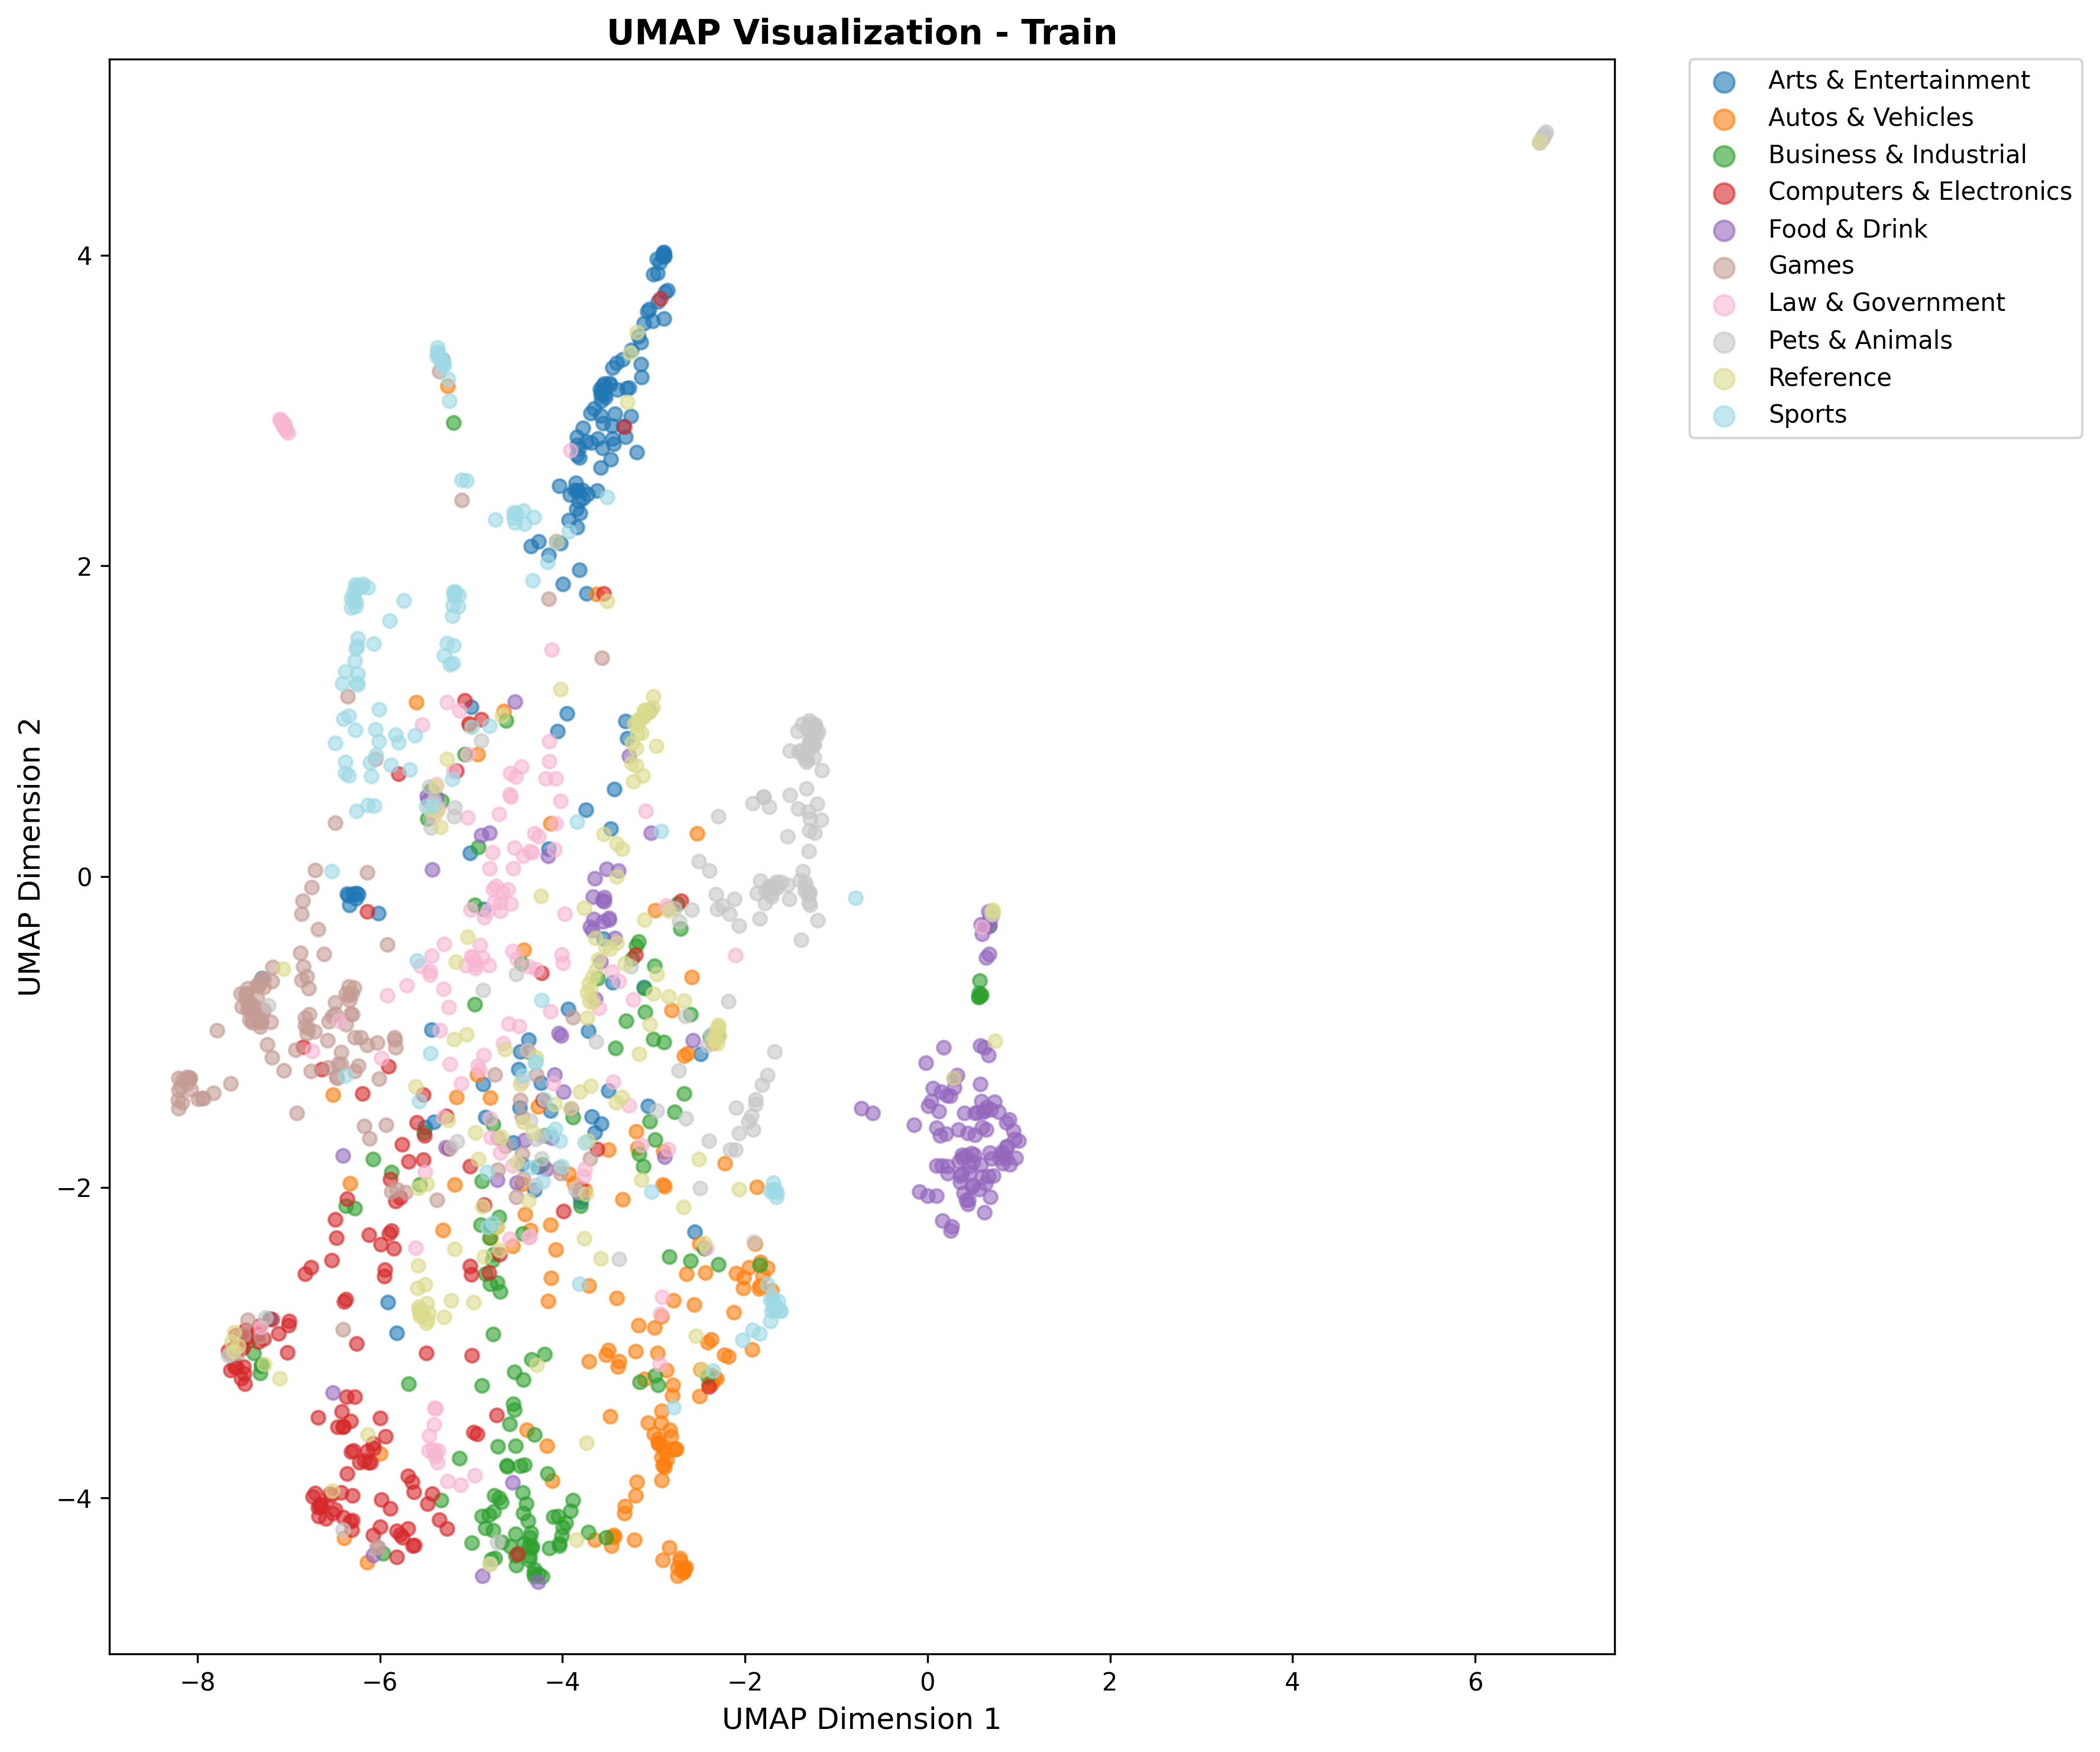
\includegraphics[width=0.8\linewidth]{asset/umap_train.png}
\caption{UMAP projection of video–text embeddings from the training set, illustrating distinct clusters for each class.}
\label{fig:umap}
\end{figure}

\subsection{Baseline Models}

%We implement two baselines for comparison:

Two baselines are implemented for the purpose of comparison:

%\begin{itemize}
    %\item \textbf{Zero-Shot Classification}: We feed the precomputed TwelveLabs video–text and text embeddings directly into a nearest-neighbor classification scheme, without any task-specific training. This approach achieves 55.6\% accuracy.
    
    %\item \textbf{TimeSformer Fine-Tuning}: We fine-tune a TimeSformer model pre-trained on Kinetics-400~\cite{kay2017kinetics} using our 1,800-video subset. After approximately 10 hours of training, this model reaches 64.0\% accuracy.
%\end{itemize}

\begin{itemize}
    \item \textbf{Zero-Shot Classification}: The precomputed TwelveLabs video-text and text embeddings are directly fed into a nearest-neighbor classification scheme, without the necessity for any task-specific training. This approach has been demonstrated to achieve an accuracy of 55.6\%.
    \item \textbf{TimeSformer Fine-Tuning}: The TimeSformer model, which has been pre-trained on Kinetics-400, is fine-tuned using a subset of 1,800 videos. Following a training period of approximately 10 hours, the model attains an accuracy of 64.0\%.
\end{itemize}

\subsection{Proposed Method}

%Our model concatenates the multimodal embeddings for each video and feeds them into a lightweight neural network consisting of:

The proposed model integrates the multimodal embeddings for each video, subsequently inputting them into a lightweight neural network comprising the following components:

%\begin{itemize}
    %\item An input layer that accepts the concatenated vector.
    %\item A Multi-Layer Perceptron (MLP) with four hidden layers (each followed by Swish activations, batch normalization, and dropout).
    %\item A final linear classification head that outputs logits over the 10 classes.
%\end{itemize}

\begin{itemize}
    \item The input layer is responsible for accepting the concatenated vector.
    \item The Multi-Layer Perceptron (MLP) layer, with four hidden layers, each of which is followed by Swish activations, batch normalization, and dropout.
    \item The final linear classification head, which generates logits for the 10 classes.
\end{itemize}

%We train for 20 epochs with a batch size of 8, using the AdamW optimizer and a CosineAnnealingLR scheduler~\cite{loshchilov2016sgdr}. On our hardware setup, total training time is approximately one minute.

The training process is conducted over a total of 20 epochs, with a batch size of 8.
The AdamW optimizer and a CosineAnnealingLR scheduler~\cite{loshchilov2016sgdr} are employed to ensure the efficient convergence of the model parameters.
The total duration of training on our hardware configuration is estimated to be approximately one minute.

%\paragraph{Embedding-Space Augmentation} To improve generalization and reduce overfitting, we apply a novel augmentation directly in embedding space. For each original embedding $\mathbf{e}$, we generate a perturbed version as follows:

\paragraph{Embedding-Space Augmentation} To enhance the generalization capabilities and mitigate the risk of overfitting, a novel augmentation technique is employed directly within the embedding space.
For each original embedding, denoted by $\mathbf{e}$, a perturbed version is generated according to the following method.
\[
\mathbf{n} = \frac{\boldsymbol{\epsilon}}{\|\boldsymbol{\epsilon}\|_2}, \quad
\boldsymbol{\epsilon} \sim \mathcal{N}(\mathbf{0},\,\mathbf{I}),
\]
\[
\mathbf{n}_{\text{scaled}} = \alpha \,\mathbf{n},\quad
\widetilde{\mathbf{e}} = \frac{\mathbf{e} + \mathbf{n}_{\text{scaled}}}{\|\mathbf{e} + \mathbf{n}_{\text{scaled}}\|_2},
\]
where \(\alpha\) is a user-defined \emph{strength} parameter. This procedure ensures that the cosine distance between \(\widetilde{\mathbf{e}}\) and \(\mathbf{e}\) is at most 
\[
1 - \sqrt{1 - \alpha^2}.
\]

%Applying Gaussian noise in this normalized way preserves the overall magnitude of the embedding while encouraging robustness to small perturbations in cosine space. Figure~\ref{fig:augmentation} illustrates the augmentation process.

The application of Gaussian noise in this normalized manner preserves the magnitude of the embedding in its entirety whilst encouraging robustness to minor perturbations in cosine space. As demonstrated in Figure~\ref{fig:augmentation}, the augmentation process is illustrated.

\begin{figure}[h]
\centering
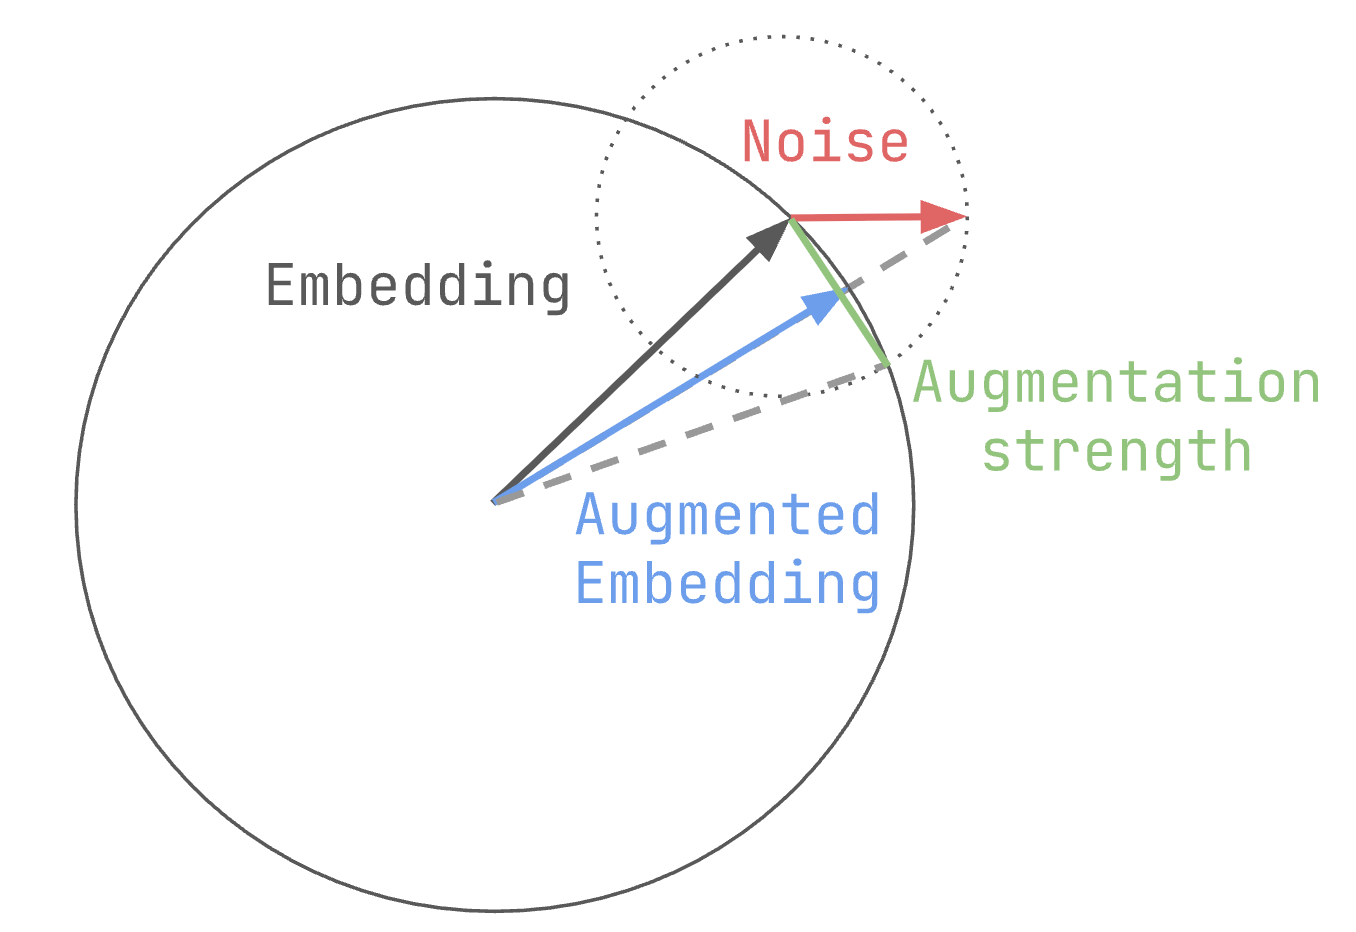
\includegraphics[width=0.6\linewidth]{asset/augmentation.png}
\caption{Schematic of the embedding-space augmentation: Gaussian noise is normalized, scaled by \(\alpha\), added to the original embedding, and then re-normalized.}
\label{fig:augmentation}
\end{figure}